%% LaTeX template for BSc Computing for Games final year project dissertations
%% by Edward Powley
%% Games Academy, Falmouth University, UK

%% Based on:
%% bare_jrnl.tex
%% V1.4b
%% 2015/08/26
%% by Michael Shell
%% see http://www.michaelshell.org/
%% for current contact information.
%%
%% This is a skeleton file demonstrating the use of IEEEtran.cls
%% (requires IEEEtran.cls version 1.8b or later) with an IEEE
%% journal paper.
%%
%% Support sites:
%% http://www.michaelshell.org/tex/ieeetran/
%% http://www.ctan.org/pkg/ieeetran
%% and
%% http://www.ieee.org/

%%*************************************************************************
%% Legal Notice:
%% This code is offered as-is without any warranty either expressed or
%% implied; without even the implied warranty of MERCHANTABILITY or
%% FITNESS FOR A PARTICULAR PURPOSE! 
%% User assumes all risk.
%% In no event shall the IEEE or any contributor to this code be liable for
%% any damages or losses, including, but not limited to, incidental,
%% consequential, or any other damages, resulting from the use or misuse
%% of any information contained here.
%%
%% All comments are the opinions of their respective authors and are not
%% necessarily endorsed by the IEEE.
%%
%% This work is distributed under the LaTeX Project Public License (LPPL)
%% ( http://www.latex-project.org/ ) version 1.3, and may be freely used,
%% distributed and modified. A copy of the LPPL, version 1.3, is included
%% in the base LaTeX documentation of all distributions of LaTeX released
%% 2003/12/01 or later.
%% Retain all contribution notices and credits.
%% ** Modified files should be clearly indicated as such, including  **
%% ** renaming them and changing author support contact information. **
%%*************************************************************************


\documentclass[journal]{IEEEtran}

\usepackage{graphicx}
\usepackage[utf8]{inputenc}
\usepackage{url}
\usepackage{amsmath}
\usepackage[]{algorithm2e}
% Insert additional usepackage commands here

\begin{document}
%
% paper title
% Titles are generally capitalized except for words such as a, an, and, as,
% at, but, by, for, in, nor, of, on, or, the, to and up, which are usually
% not capitalized unless they are the first or last word of the title.
% Linebreaks \\ can be used within to get better formatting as desired.
% Do not put math or special symbols in the title.
\title{Extending Client Side Prediction Methods in Networked Multiplayer First Person Shooter Games to Include Game State Information}
%
%
% author name
\author{Richard Steele}

% The paper headers -- please do not change these, but uncomment one of them as appropriate
% Uncomment this one for COMP320
\markboth{COMP320: Research Review and Proposal}{COMP320: Research Review and Proposal}
% Uncomment this one for COMP360
% \markboth{COMP360: Dissertation}{COMP360: Dissertation}

% make the title area
\maketitle

% As a general rule, do not put math, special symbols or citations
% in the abstract or keywords.
\begin{abstract}
This paper critically examines the effectiveness of the current methods of client side prediction in networked multiplayer digital games, specifically first person shooter games where the accuracy of each game agent's behaviour is critical to the player's experience. The de facto use of \textit{dead reckoning} is accepted as a standard tool to help minimise the number of required network updates, but its results can be error prone which are a detriment to the player's experience. This paper looks at the currently used dead reckoning algorithms and suggests using further data about the game state to provide a more accurate estimation of a game agent's location and behaviour at a future time. Knowledge about the layout of a level is used to dynamically alter the threshold of the dead reckoning algorithm's allowance to better reflect an agent's behaviour at critical points of the game by sending an increased amount of player updates.
\end{abstract}

\section{Introduction}
% The very first letter is a 2 line initial drop letter followed
% by the rest of the first word in caps.
% 
% form to use if the first word consists of a single letter:
% \IEEEPARstart{A}{demo} file is ....
% 
% form to use if you need the single drop letter followed by
% normal text (unknown if ever used by the IEEE):
% \IEEEPARstart{A}{}demo file is ....
% 
% Some journals put the first two words in caps:
% \IEEEPARstart{T}{his demo} file is ....

\IEEEPARstart{W}{ith} modern networked multiplayer digital games where the game state must be updated often, it is impractical to send and receive network updates on every frame. Instead, \textit{dead reckoning} algorithms are used to predict future states of the game, and network updates are needed only when the actual behaviour differs from the predicted behaviour by a threshold amount. This idea of an acceptance threshold accepts that the perception of an entity for all other clients on a network may differ to the actual state of that entity. While effective at greatly reducing the required network updates and reducing the impact of network transmission delay \cite{pantel2002suitability}, impossible behaviours such as tunnelling (projecting a position past a barrier), or improbable behaviours counter intuitive to the game are possible. This paper proposes that by using further information about the game state, such as level layout, an agent's behaviour can be predicted with greater accuracy to help minimise unwanted behaviour.

Previous papers in the context of games describe dead reckoning as a measure to account for network latency compensation. Few expand beyond this and are concerned generally with how best to marry the predicted state with the actual state by interpolation or rolling back. This paper explores improving the accuracy of the simulation by dynamically adjusting the threshold allowed by traditional dead reckoning methods to prompt more frequent state updates at critical times when the greatest accuracy is required.

It is important to note that not all networked multiplayer games suffer from client side prediction problems. For instance turn based games consider each client sequentially. Where there is no scope or benefit for a player to react immediately, no measures must be taken to account for problems incurred by some milliseconds lost in transmission. These issues are prevalent in fast paced competitive games such as racing games, or the first person shooter genre. This paper then bases its study upon the first person shooter game genre, sometimes referred to as \textit{twitch} shooters \cite{lee2015outatime}. The need to respond quickly to other clients' perceived actions is critical to the player experience, therefore it is crucial that those actions are shown as accurately as possible.

The research question that this paper addresses is: how can client side prediction in networked multiplayer first-person shooter games that use dead reckoning be improved?

\section{Background}

This literature review first confirms the definition of client side prediction, the problems that it solves, and the trade off against absolute accuracy. Dead reckoning is explained and explored with a focus on the real world applications and techniques of its use within games. Finally, alternative methods of solving the the problems associated with network latency are explained and acknowledged.

\subsection{Client side prediction}

Networked multiplayer games are defined as sharing a game space between multiple clients \cite{diot1999distributed}. Each client holds a representation of that game space which it uses to display information to the user, and allows the user to change within the rules of the game. When elements or details of the agents of that game space are changed by a client's actions, the client assumes that the action is successful, performs that action on its own game state representation, then sends the action information to the network so as all other clients can update their own game space representation to reflect the performed action \cite{bernier2001latency}.

Problems can occur when:
\begin{itemize}
    \item the updated information is received too late (network latency)
    \item the updated information is not received (packet loss)
    \item the action is not successful (simultaneous conflicting actions are performed by many clients).
\end{itemize}

Network latency forms the primary bottleneck for online game performance with an acceptable value being under 100 milliseconds \cite{lee2015outatime} \cite{smed2002aspects} and worst case overall latencies claimed to be up over 1 second \cite{claypool2006latency}. To counter this, each client takes the slightly old network state update that it receives and brings it approximately up to date through extrapolation before displaying it to the user. Performance degrades significantly under variance in latency (or \textit{Jitter}) \cite{beigbeder2004effects} \cite{dick2005analysis}. The jitter effect must be continually accounted for as the delta time value between updates can be subject to change. As such, the current time in which an action is performed is included with the update packet of data sent and received by clients, and forms an integral part of the prediction algorithm. The latency time difference must be continuously evaluated by sending and receiving time stamped packets to maintain a correct delta time value \cite{glazer2015multiplayer}, however manipulating these time stamps is an opportunity for cheating \cite{jamin2003cheat} so must be secure from interference or if using a centralised server then a globally synchronised clock can be used \cite{aggarwal2004accuracy}.

Given the vast quantity and unreliable nature of the messages being sent \cite{cronin2001distributed}, packet loss must be planned for. The same dead reckoning methods used to account for network latency, and outlined in \textit{B.} can be used to replace missing packets of information, or application data units (ADUs) \cite{diot1999distributed} sometimes referred to as protocol data units (PDUs) \cite{dis1998ieee}, to supply a prediction of where the ADU's agent will ``most probably'' be at a given time.

\subsection{Dead reckoning}

Dead reckoning methods are based on a navigational technique of estimating one’s position based on a known starting point and velocity \cite{smed2002aspects}. In the simplest implementation, we take the last position we received on the network, and project it forward in time with at its last known velocity \cite{murphy2011believable}.

\begin{figure}[h]
    \centering
    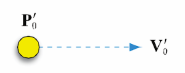
\includegraphics[width=0.5\linewidth]{DR1.png}
    \caption{Image sourced from \cite{murphy2011believable}}
    \label{fig:dr1}
\end{figure}

This simple representation of projecting forward is correct if an agent has linear movement and constant velocity. However, agents in a first person shooter game often have complex non linear movements which will need to be checked for and accommodated. Real world applications of linear dead reckoning also suffer with having to account for unpredictable behaviour e.g. drift due to wind or wheel slippage \cite{chung2001accurate} \cite{ojeda2004experimental}. The techniques used for managing these behaviours are transferable to the problems of dead reckoning networked multiplayer game agents with complex behaviour.

In 1983, with substantial support from the U.S. army, the Defense Advanced Research Projects Agency (DARPA) initiated the Simulator Networking (SIMNET) program which developed dead reckoning techniques to support a virtual world to train soldiers \cite{calvin1993simnet}. Their approach to networking solutions has been incorporated into the Distributed Interactive Simulation (DIS) standard which is now an IEEE standard \cite{dis1998ieee}. It outlines the use of a PDU to help dead reckoning handle complex behaviour \cite{mccarty1994virtual}. It is worth remembering however that DIS was designed for use by a small number of players (less than 50), and the inclusive PDU model can be criticised for holding too much redundant data \cite{henderson2001latency}.
 
Each client maintains a dead reckoned model of itself that corresponds to the model used by other clients to ``see'' its represented agent. The client must regularly check whether the difference between the predicted state calculated with dead reckoning that all clients share and the actual state exceeds a certain threshold. If this is the case, the client is then responsible to generate an updated entity state for the dead reckoning algorithm to apply to the model. Then send that updated state to all clients on the network to learn about the correct new state of the entity to then use to update their own model of that client's agent \cite{calvin1993simnet} \cite{mauve2000keep}. This also happens when a fixed amount of time has passed since the last update (normally 5 seconds) \cite{mills1992network}.

\begin{figure}[h]
    \centering
    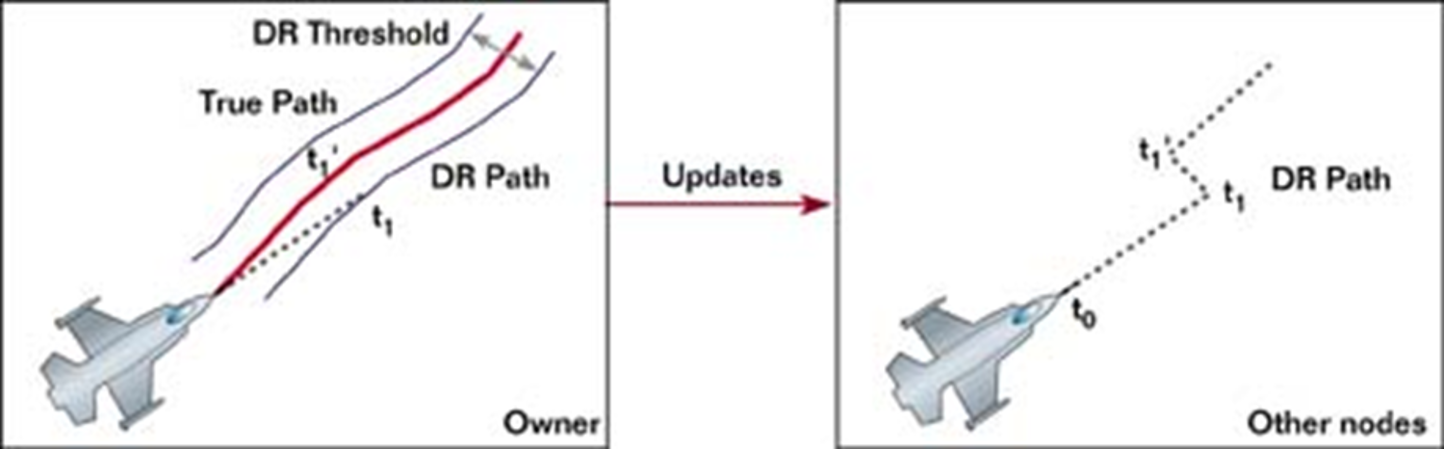
\includegraphics[width=0.7\linewidth]{Threshold1.png}
    \caption{Image sourced from \cite{aronson1997gamasutra}}
    \label{fig:threshold}
\end{figure}

Were this updated information used immediately, the modelled entity would appear to jump (fig. \ref{fig:threshold}). Instead, the dead reckoning algorithm uses interpolation and projective velocity blending \cite{murphy2011believable} to tend towards and eventually reconcile its own dead reckoned model with the newly updated state information (fig. \ref{fig:dr2}, fig. \ref{fig:dr3}).

\begin{figure}[h]
    \centering
    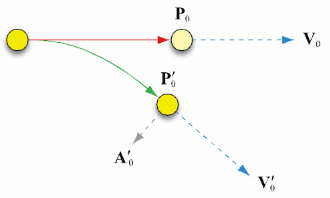
\includegraphics[width=0.7\linewidth]{DR2.png}
    \caption{Image sourced from \cite{murphy2011believable}}
    \label{fig:dr2}
\end{figure}

\begin{figure}[h]
    \centering
    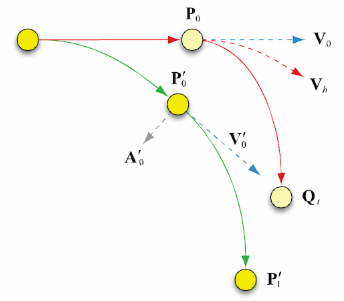
\includegraphics[width=0.7\linewidth]{DR3.png}
    \caption{Image sourced from \cite{murphy2011believable}}
    \label{fig:dr3}
\end{figure}

\begin{align}
        Q_t & = {P'_0} + {V'_0} T + \frac{1}{2} {A'_0} T^2 \\
        V_b &= V_0 + ({V'_0} - {V_0}) \Hat{T}  \\
        P_t &= P_0 + {V_b}{T_b} + \frac{1}{2} {A'_0} {T_t^2}  \\
        P'_t &= {P'_0} + {V'_0}{T_t} + \frac{1}{2}{A'_0}{T_t^2}\\
        Q_t &= P_t + ({P'_t} - P_t ) \Hat{T} 
\end{align}

\cite{murphy2011believable} \\ \\
(1) Linear dead reckoning as shown in fig \ref{fig:dr1}. $P'_0$ is the initial position of the entity. $V'_0$ is its velocity. $A'_0$ is its acceleration. $Q_t$ is its dead reckoned position at time $T$.  \\ \\
(2) etc... Projective velocity blending as shown in fig \ref{fig:dr2} and fig \ref{fig:dr3} \\ \\
(3) \\
(4) \\
(5) \\

(Explain equations here)

It has been shown that using derivatives of orders higher than two usually results in a negligible improvement in the prediction [8, 9]. As a result, the use of first and second order derivatives is usually preferred and estimating the velocity and acceleration and sending them with the current position is sufficient for short-term dead reckoning \cite{yahyavi2011antreckoning}

dynamic equations of motion

Newton's second law which links the \textit{acceleration} of an object, its \textit{mass}, and the \textit{forces} it is subject to (1).

\begin{algorithm}
\DontPrintSemicolon % Some LaTeX compilers require you to use \dontprintsemicolon instead
\KwIn{ \\ prediction error threshold: $\eta$ \\ last time a position was sent: $t_o$ \\ actual position (at time $t$): $x_t$}
$t_0 \gets -\infty$\;
\ForEach{frame (time $t$)}{
  $\Hat{x}_t \gets$ prediction($x_{t_0}, t$);\;
    \If{$||x_t - \Hat{x}_t|| > \eta $}{
        send(x_t)\\
        $t_0 \gets t$\;
    }
}
\caption{Threshold based dead reckoning: a player predicts the position of their agent for the current frame, based on the last sent position update, sending an update only if the prediction error is larger than a threshold $\eta$}
\label{algo:pseudo}
\end{algorithm}

\subsection{Interest modelling}

The shortcomings of estimating a game player's behaviour based only upon motion dynamics are already recognised. Amir Yahyavi \textit{et al} successfully use identified points of interest to influence their dead reckoning algorithm, improving the accuracy by up to 30\% over traditional dead reckoning techniques \cite{yahyavi2011antreckoning}. They propose the use of \textit{attraction forces}, derived from the player state and nearby points of interest, to be factored into the dead reckoning calculation alongside the current acceleration. The example that they cite is that a player controlling an entity with reduced health will most likely move towards a health pack if there is one in sight. However, their method titled \textit{AntReckoning} must decide on the attraction forces of each point of interest, to build a \textit{pheromone map}. The reliability of this can be disputed as different players will have differing goals, but the increase in accuracy reported is excellent. The merit of Amir Yahyavi's work \cite{yahyavi2011antreckoning} \cite{yahyavi2013interest} \cite{yahyavi2013towards} recognising and proposing solutions to the problems of solely using traditional dead reckoning methods in games with client side prediction is acknowledged and an inspiration for this project.

\cite{yahyavi2013interest}

\cite{yahyavi2013towards}

\cite{cai1999auto}

\cite{jaya2016combining}

\cite{larsson2016movement}

\subsection{Heat maps}

As common to most games, AntReckoning assumes
a game world divided into non overlapping cells,
e.g., Delaunay triangulation, Voronoi tessellation, binary space
partitioning, or regular grids (e.g., square grid in Figure 1)

\cite{bauckhage2014beyond}

\cite{kuipers1978modeling}

\cite{wilkinson2009history}

\cite{moumtzidou2013discovery}

\cite{drachen2013spatial}

Finally, to visualise the level data that this project uses to adjust it's client side prediction request rate...

to aggregate PDU states at critical junctions

Using game state information to adapt client side prediction is still in its infancy.


\subsection{Discussion}

The two part purpose of client side prediction is to maintain an up to date game state for clients in the case of late or lost packets, and to use prediction algorithms to reduce required network updates. A distributed virtual environment (DVE) could further reduce packet updates by filtering for an area of interest. Only sending a client's information for entities that are within that player’s potential field of sight \cite{cronin2001distributed}. However, this requires previous knowledge of all entity positions therefore a two pass approach would be needed to determine which entities would be affected by a state change, and then to update those clients. This \textit{relevance filtering} is reliant upon a \textit{radius of interest} \cite{rak1996evaluation}.  We acknowledge this method's effectiveness in specific situations to reduce network updates. But, given the often edge to edge viewing range prevalent in many game levels \cite{toby2014tobyscs} \cite{ziervogel2014nag} \cite{cod2018wikibo4}, this paper argues against its use in a general approach to improving client side prediction in first person shooter games.

Laurent Gautier and Christophe Diot propose that late packets due to network latency may be accommodated by the client by introducing a local presentation delay to provide a consistent, distributed state \cite{gautier1998design}. However, these increase the application-level delay even more so. While acceptable for their MiMaze maze navigation project, it is unsuitable for the fast paced style of first person shooter games.

While the simplest dead reckoning algorithm provides a linear vector approximation based on velocity, we have shown above that interpolation and projective velocity blending can be used to smooth trajectories between state updates tending towards the correct representation. James M. Van Verth and Lars M. Bishop provide a method to sample and project cubic bezier spline curves \cite{van2008essential} but these are shown to be slightly less accurate than the velocity blending technique shown above proposed by Curtiss Murphy \cite{murphy2011believable}. It is a fundamental requirement for believable games that the state transitions are smooth and believable, which is why curves are employed rather than a jump. These curves are shown to be accurate when inferred from polynomial modelling based on the Lagrange or Taylor series \cite{hanawa2006proposal}. But require multiple states from which to extrapolate an approximation. Packet loss can be greatly detrimental to this approach. Small sample sizes combined with potentially erratic movement of game players will likely produce unlikely results. For instance player’s could turn instantaneously and apply unrealistic forces to create huge accelerations at arbitrary angles \cite{bernier2001latency}. A solution would be to provide back up copies of previous states in each PDU to restore missing information. A technique already employed in Quake where the last three commands are also sent in each packet to compensate for lost packets \cite{cronin2001distributed}.

Dead reckoning is an \textit{optimistic algorithm}. It assumes it is correct  and when it is not, it must adjust itself. It is apparent that the blending of this adjustment may result in compromising behaviour. Demonstrated in first person shooter games as appearing to other players in a vulnerable position outside of cover, or moving through an impenetrable area as defined by the game's movement rules.

The de facto method of dead reckoning entities' behaviours is a distributed approach that does not require a centralised server. Using a distributed approach is mandatory for many DVEs in order to avoid the well known problems of centralised systems such as increased latency, single-point-of-failure and lack of scalability \cite{mauve2000keep}. However, having a dedicated central authoritative server (or a single client nominated as such) means that even if a client simulates different results than the server, the server’s results will eventually correct the client’s incorrect simulation \cite{bernier2001latency}

as proposed by \textit{AntReckoning} \cite{yahyavi2011antreckoning}

Donnybrook protocol looks to increase the delay between packets up to seconds

the threshold above which a new update is sent is adapted to the precision requirements, determined by the relative position of the entities \cite{cai1999auto} - Looks to reduce the number of update packets, whereas this project considers increasing them for small scale multiplayer games

neural networks are trained and used, instead of instantaneous estimates, to predict changes of the entity velocity \cite{mccoy2007multistep}

----------------------------------

Motivated by this ...


The literature shows a broad ...

The challenges are ...

This project attempts to focus current methods into ... more game related where information about the game state are globally known



Talk about trade off

network latency would cause the received data to be slightly behind,

Leading a shooting mechanic to account for lag \cite{bernier2001latency}

smooth trajectories between state updates, and also decrease the frequency of state transmission.

allows to prolong the interval of message transmissions and abolish the network latency at the cost of data consistency \cite{smed2002aspects}

In the case of lost packets resulting in no update data for that agent. Instead, dead reckoning methods are used to simulate an agent's behaviour, allowing client-side prediction to reduce the impact of a network transmission delay \cite{pantel2002suitability}. When used effectively this can help to synchronise the game state across all clients.


% this paper looks good to cite for explanation of dr


Buckets or late updates may lead to repairing inconsistencies requiring a rollback which will cause more drastic position jumps \cite{cronin2002efficient}

Previous synchronisation mechanisms such as bucket synchronisation and Time Warp are not well suited to the demands of a real-time multiplayer game. Trailing state synchronisation is designed specifically for real-time multiplayer games, and achieves better responsiveness and scalability while maintaining near-perfect consistency \cite{cronin2001distributed}

Commercial context - why important to have good solutions of the problem - see reviews? Metacritic

Context for problem space

A lot of fps have problems because of network problems, find reviews, quote popularity. See criticism.spread the assumptions across white and grey. Pull in grey lit and peer review. \cite{solaire2016reddit} \cite{hp2015bungie}


Discuss state conflicts





\section{Methodology}

Time. Is on my side, oh yes it is.


% references section

\bibliographystyle{IEEEtran}
\bibliography{references}

% Appendices

%\appendices
%\section{First appendix}
%Appendices are optional. Delete or comment out this part if you do not need them.

% that's all folks
\end{document}


Describe state of field in relation to literature

Define the problem, grey lit for dead man can shoot gamasutra etc

find papers and authors that support the position I'm taking.



practical motivation

Academic motivation

Gaps in literature
Dead reckoning algorithms only use information on the player's current and simulated location and velocity.

tunnelling problem
co cognition
bots but intent needs to be carried across



what is dr

why have dr

how when where

What is good about it 
What problems does it solve
strengths

What is bad about it
weaknesses
is it a problem

propose solution